\documentclass[a4paper, 10pt]{article}

\usepackage[margin = 1in]{geometry} % for spacing around
\usepackage{graphicx} % for including images in your pdfs
\usepackage{xcolor} % for including colors in your pdf
\usepackage{soul} % for text decoration
\usepackage[utf8]{inputenc} % for encoded text
\usepackage[T1]{fontenc}
\usepackage{setspace} % for setting different line spacings between paragrafs.
\usepackage{enumerate} % for letting us get more detailed enumerate lists
\usepackage{multirow} % to let us combine more rows together
\usepackage{colortbl} % for decorating tables
\usepackage{amsmath} % used for representing more complicated math displays
\usepackage{supertabular}
\usepackage{longtable} % both of these packages are used to making really big tables
\usepackage{wrapfig} % allows us to wrap text around figures
\usepackage{fancyhdr} % for making fancy headers
%\usepackage{bibtex} % for making better bibliographies
\usepackage[pdftex]{hyperref} % for letting us make links
\usepackage{lscape} % Allows us to flip from portrait to landspace
\usepackage{tikz} % for high detailed drawing
\usepackage{multicol} % To put things side by side
\usepackage{rotating} % For rotating objects
% \usepackage{draftwatermark} % For adding watermarks
\usepackage{MnSymbol} % for using multiple symbols
\usepackage{mathtools} % Used for more math symbols
\usepackage{xfrac} % For more complciated fractions and to add derivitives
\usepackage{hyperref} % for hyper links
\usepackage{enumitem} % for better enum lists
\usepackage{tcolorbox} % for adding colored text boxes
\usepackage[framed,numbered,autolinebreaks,useliterate]{mcode} % for including mathlab code
\usepackage{bm} % Adding bold text to math inputs

% Setting up the default image path
\graphicspath{{./Pictures/}}

% Implementing authro details
\title{Solutions for Homework14}
\author{Emre Arapcic-Uvak & Vedad Siljic}
\date{}

% Setting up the fancy page style
\fancypagestyle{customStyle}{
	\lhead{} \chead{} \rhead{}
	\lfoot{} \cfoot{\thepage} \rfoot{}
	\renewcommand{\headrulewidth}{0pt}
	\renewcommand{\footrulewidth}{1pt}
}
\pagestyle{customStyle}

% Setting up hyperref options
\hypersetup {
	colorlinks = false,
	citecolor = black,
	filecolor = blue,
	linkcolor = blue,
	urlcolor = blue,
	pdftex
}

% Custom commands
\newcommand{\important}[1]{\textcolor{red}{\textbf{\textsc{#1}}}}
\newcommand{\miniHeader}[1]{\begin{large}\textbf{\textsc{#1}}\end{large}}
\newcommand{\volumeUnit}[0]{\frac{g}{cm^{3}}}

\begin{document}
	\maketitle
	\vspace{5mm}
	
	\begin{abstract}
		\begin{center}
			\noindent In this document we will show the solutions for problems represented in the given homework for this week.
		\end{center}
	\end{abstract}
	\pagebreak
	
	\tableofcontents
	\pagebreak
	
	\section{Task 1}
	
		\subsection{Problem}
			\noindent In the given graph which represents the movement of a car, answer the following:
			\begin{itemize}
				\item Between which point and point the car accelerate, and between which points it decelerate?
				\item What is the distance traveled at point C? and what is it at point F?
				\item Indicate line segments with 0 acceleration, does that mean the car is not moving? Explain.
				\item What are the values of acceleration and deceleration of the car at each segment?
			\end{itemize}	
		
			\begin{figure}[h]
				\centering
				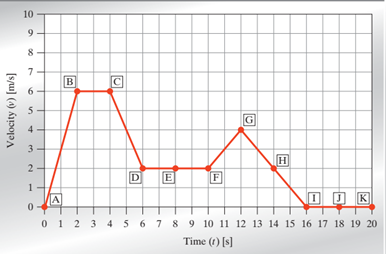
\includegraphics{Task1CarVelocityTimeGraph}
				\caption{Velocity-Time of the car}
				\label{fig:task1Fig}
			\end{figure}
		\subsection{Solution}
			\begin{enumerate}
				\item 
					\noindent The car accelerates at points:
					\begin{itemize}
						\item $A \rightarrow B$
						\item $F \rightarrow G$
					\end{itemize}
				
					\noindent And it decelerates at points:
					\begin{itemize}
						\item $C \rightarrow D$
						\item $G \rightarrow I$ ($G \rightarrow H$ \& $H \rightarrow I$)
					\end{itemize}
				\item 
					To get the distance we can just find the integral from point $A$ (0) to whatever points we want. So to see what the distance traveled at point $C$ is we just have to evaluate \[\int_{A}^{C}v*dt = \int_{A}^{B}v*dt + \int_{B}^{C}v*dt\]which is just the area under the graph so from $A \rightarrow B$ we have a right triangle with sides $1 \times 6$ which means that the area from that triangle is $\frac{6}{2} = 3$, and from $B \rightarrow C$ we have a rectangle with sides $2 \times 6$ so in total the area of the rectangle is $12$ meaning that the distanced traveled from $A \rightarrow C$ is $3 + 12 = 15m$. To find out the distance traveled from $A \rightarrow F$ we have to solve the following integral: \[\int_{A}^{F}v*dt = \int_{A}^{C}v*dt + \int_{C}^{B}v*dt + \int_{D}^{F}v*dt\]
					Since we already know that $\int_{A}^{C}v*dt = 15m$ we just have to find the other two integrals, which at the end end up being $15 + \frac{2*4}{2} + 2*2 + 2*4 = 15 + 4 + 4 + 8 = 31m$
				\item 
					The line segments with $0$ acceleration are
					\begin{itemize}
						\item $B \rightarrow C$
						\item $I \rightarrow K$ ($I \rightarrow J$ \& $J \rightarrow K$)
					\end{itemize}
					This does \textcolor{red}{\textsc{not}} mean that the car isn't moving, this just means that the velocity of the car isn't changing or in other words \[\frac{dv}{dt} = 0\]
				\item 
					\vspace{5mm}
				{
					\centering
					\begin{tabular}{|c|c|}
						\hline \hline 
						\textsc{Line Segment} & \textsc{Acceleration value $\left[\frac{m}{s^2}\right]$} \\ \hline
						$A \rightarrow B$ & 3 \\ \hline
						$B \rightarrow C$ & 0 \\ \hline
						$C \rightarrow D$ & -2 \\ \hline
						$D \rightarrow E$ & 0 \\ \hline
						$E \rightarrow F$ & 0 \\ \hline
						$F \rightarrow G$ & 1 \\ \hline
						$G \rightarrow H$ & -1 \\ \hline
						$H \rightarrow I$ & -1 \\ \hline
						$I \rightarrow J$ & 0 \\ \hline
						$J \rightarrow K$ & 0 \\ \hline \hline
					\end{tabular}
					\par
				}
			\end{enumerate}
	\section{Task 2}
	
		\subsection{Problem}
			\noindent An environmental engineer has obtained a bacteria culture from a municipal water sample and allowed the bacteria to grow. The initial count of Bacteria is A, and their growth formula with time being in hours is given by: \[B = B_{0}e^{Ct}\]
			
			\noindent A: is the summation of your birthday digits divided by 0.5 \\
			\noindent C: is the summation of your IUS ID number divided by 50.
			
			\begin{itemize}
				\item What is $B_0$? And what is its value?
				\item After how many hours, the amount of Bacteria would be 100000?
				\item Pick up 4 to 5 points in time and draw the graph of Bacteria growth. (This is done by pen and pencil)
				\item Use Octave to plot the graph of bacteria growth 
			\end{itemize}
			\pagebreak
			
		\subsection{Solution}
			\[A = \frac{1 + 4 + 1 + 2 + 2 + 0 + 0 + 2}{0.5} = \frac{12}{0.5} = 24\]
			\[C = \frac{2 + 2 + 0 + 3 + 0 + 2 + 2 + 8 + 9}{50} = \frac{28}{50} = 0.56\]
			
			\begin{enumerate}
				\item 
					$B_0$ is the initial amount of bacteria in our system and since our variable $A$ represents the initial count of bacteria we can conclude that $A = B_0$.
				\item 
					To figure this out we simply have to figure out the following equation:
					\[24*e^{0.56*t} = 100000\] \[0.56*t*\ln{24*e} = \ln{100000}\] 
					\[0.56*t = \frac{\ln{100000}}{\ln{24*e}}\]
					\[t = \log_{24*e}{100000} * \frac{1}{0.56}\]
					\[t \approx 4.9207 [h]\]
				\item 
					Using the following code:
					\lstinputlisting{./OctaveCode/BacterialGrowthPlot.m}
					
					\noindent We get the following graph
					\begin{figure}[h]
						\centering
						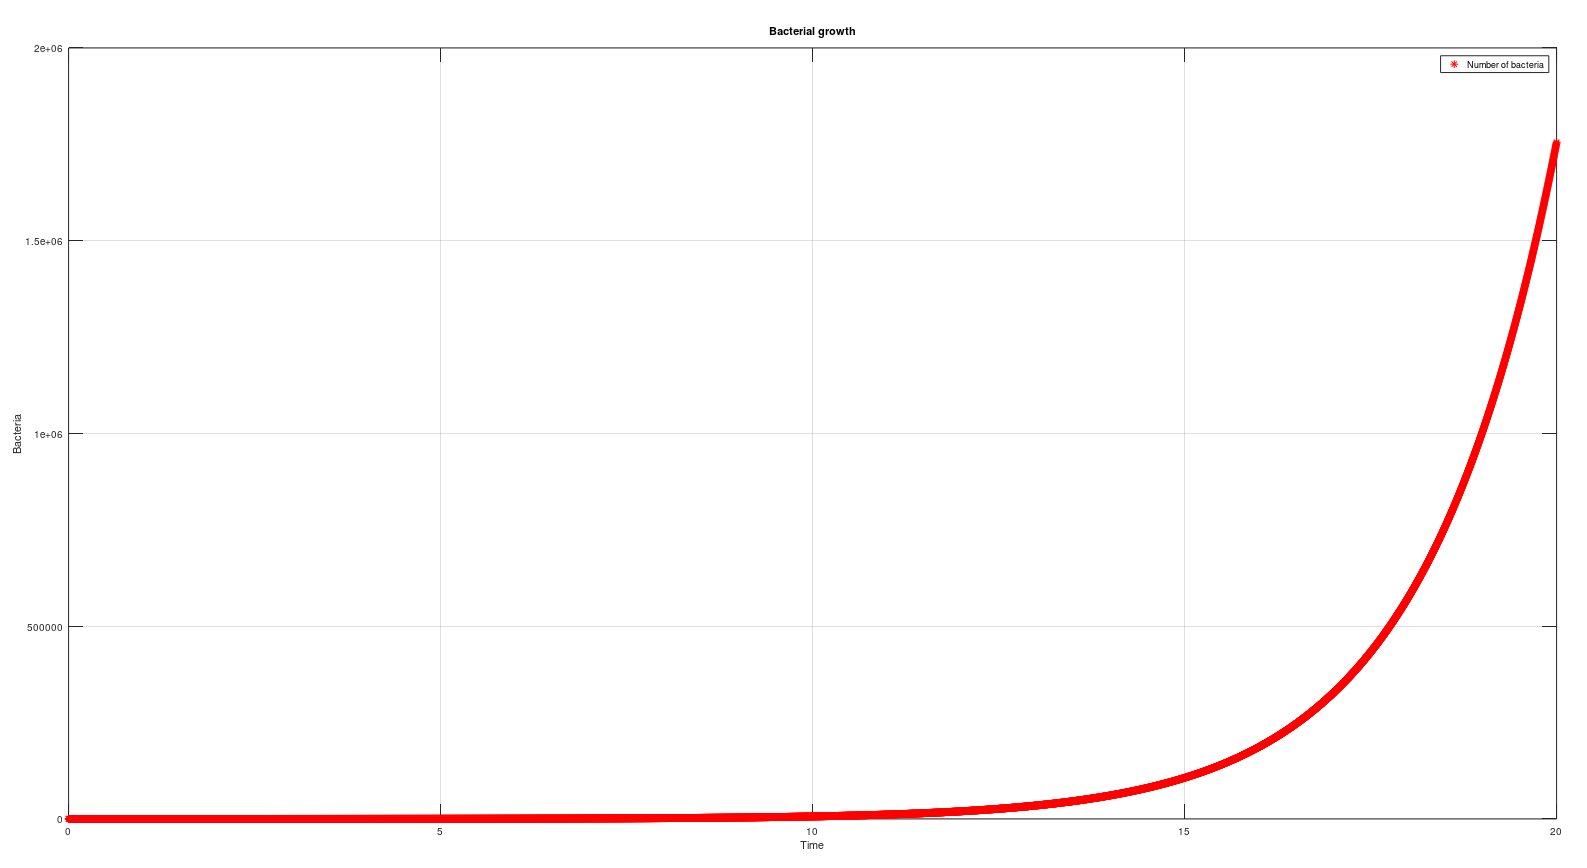
\includegraphics[scale = 0.33]{BacterialGrowthGraph}
						\caption{Bacterial growth plot}
						\label{fig:bacterialGrowth}
					\end{figure}
			\end{enumerate}
	\section{Task 3}
	
		\subsection{Problem}
		
		\subsection{Solution}
	
	\section{Task 4}
	
		\subsection{Problem}
			\begin{enumerate}
				\item
					\noindent Consider the following loop:
					\lstinputlisting{./OctaveCode/Task4Problem1.m}
					
					\noindent If we were to run the code and generate the following value for T, T = [2 11; 7 16]. What is D
				\item 
					What is the output of $M4$ if M = [1 3 2; 6 0 2]
					\lstinputlisting{./OctaveCode/Task4Problem2.m}
			\end{enumerate}
		\subsection{Solution}
			\begin{enumerate}
				\item 
					If we take a good look at the code we can spot that the first element is always going to be the element on the main diagonal line of the matrix, and the 2nd element will always be the element of the inverse diagonal of the matrix so if we get T = [2 11; 7 16]. D must be:
					\[D = \begin{bmatrix}
						2  & 7 \\
						16 & 11
					\end{bmatrix}\]
				\item 
					All this code does is take the number of rows and columns, afterwards if makes loops that repeat twice the number of rows and columns. So for a $2 \times 3$. We would have in total 24 itterations. The final output would be:
					\[M4 = \begin{bmatrix}
						1  & 2 & 3 & 4 & 5 & 6 \\
						1  & 2 & 3 & 4 & 5 & 6 \\
						1  & 2 & 3 & 4 & 5 & 6 \\
						1  & 2 & 3 & 4 & 5 & 6 
					\end{bmatrix}\]
					
			\end{enumerate}
		\pagebreak
	\section{Task 5}
	
		\subsection{Problem}
			\noindent Write a program that will ask the user to input his age in year and it will calculate to him his age in days.
		\subsection{Solution}
			\lstinputlisting{./OctaveCode/AgeCalculator.m}
	\section{Task 6}
	
		\subsection{Problem}
			\noindent Write a program that takes a vector as it’s input and returns the maximum, minimum, and mean of the given vector. And it returns how many positive, negative and 0 numbers in the vector as well.
		\subsection{Solution}
			\lstinputlisting{./OctaveCode/vectorScrutinizer.m}
	\section{Task 7}
	
		\subsection{Problem}
		
		\subsection{Solution}
	
	\section{Task 8}
	
		\subsection{Problem}
		
		\subsection{Solution}
	
	\section{Task 9}
	
		\subsection{Problem}
		
		\subsection{Solution}
	
	\section{Task 10}
	
		\subsection{Problem}
		
		\subsection{Solution}
\end{document}